% !TEX root = 99_main.tex

The parametric design environment (PDE), shown schematically in Figure \ref{fig:performative} details the multiple processes that were used in parallel to handle the different technological branches. From this, four key outputs are generated: the structural performance, energetic performance, manufacturing plans, and visual renders. Inputs to the PDE are defined by the parameters that have the greatest influence on the design. In this case, they are the overall frame dimension and profile, the photovoltaic panel dimension, spacing and layout, and the range of motion. 

These inputs are numerically fed into the design environment and generate instantaneous results of the structural performance, energetic performance, visual renders and manufacturing plans. By doing so, the multiple tradeoffs between the technological branches, as explained in Section \ref{ch:introduction1}, can be simulatenously observed. The electricity generation, building energy demand, utilisation factor of yield strength, dimensions, collision detection, aesthetics, and manufacturing costs are of particular interest. This ultimately allows for quick feedback loops with the major stakeholders (architects, structural engineering, energy engineers, and production team) involved in the project. \\


The environment combines the geometric modelling software Rhinoceros 3D \cite{Rhino}, its parametric plug-in Grasshopper \cite{grasshopper}, and python \cite{python} as a scripting language. The relatively unspecialised nature of Rhino is complemented by a large number of specialised add-ons for Grasshopper. Furthermore, custom Grasshopper modules can be scripted using python. The following subsections will explain the structural and energetic analysis in more detail.

\begin{figure}
\begin{center}
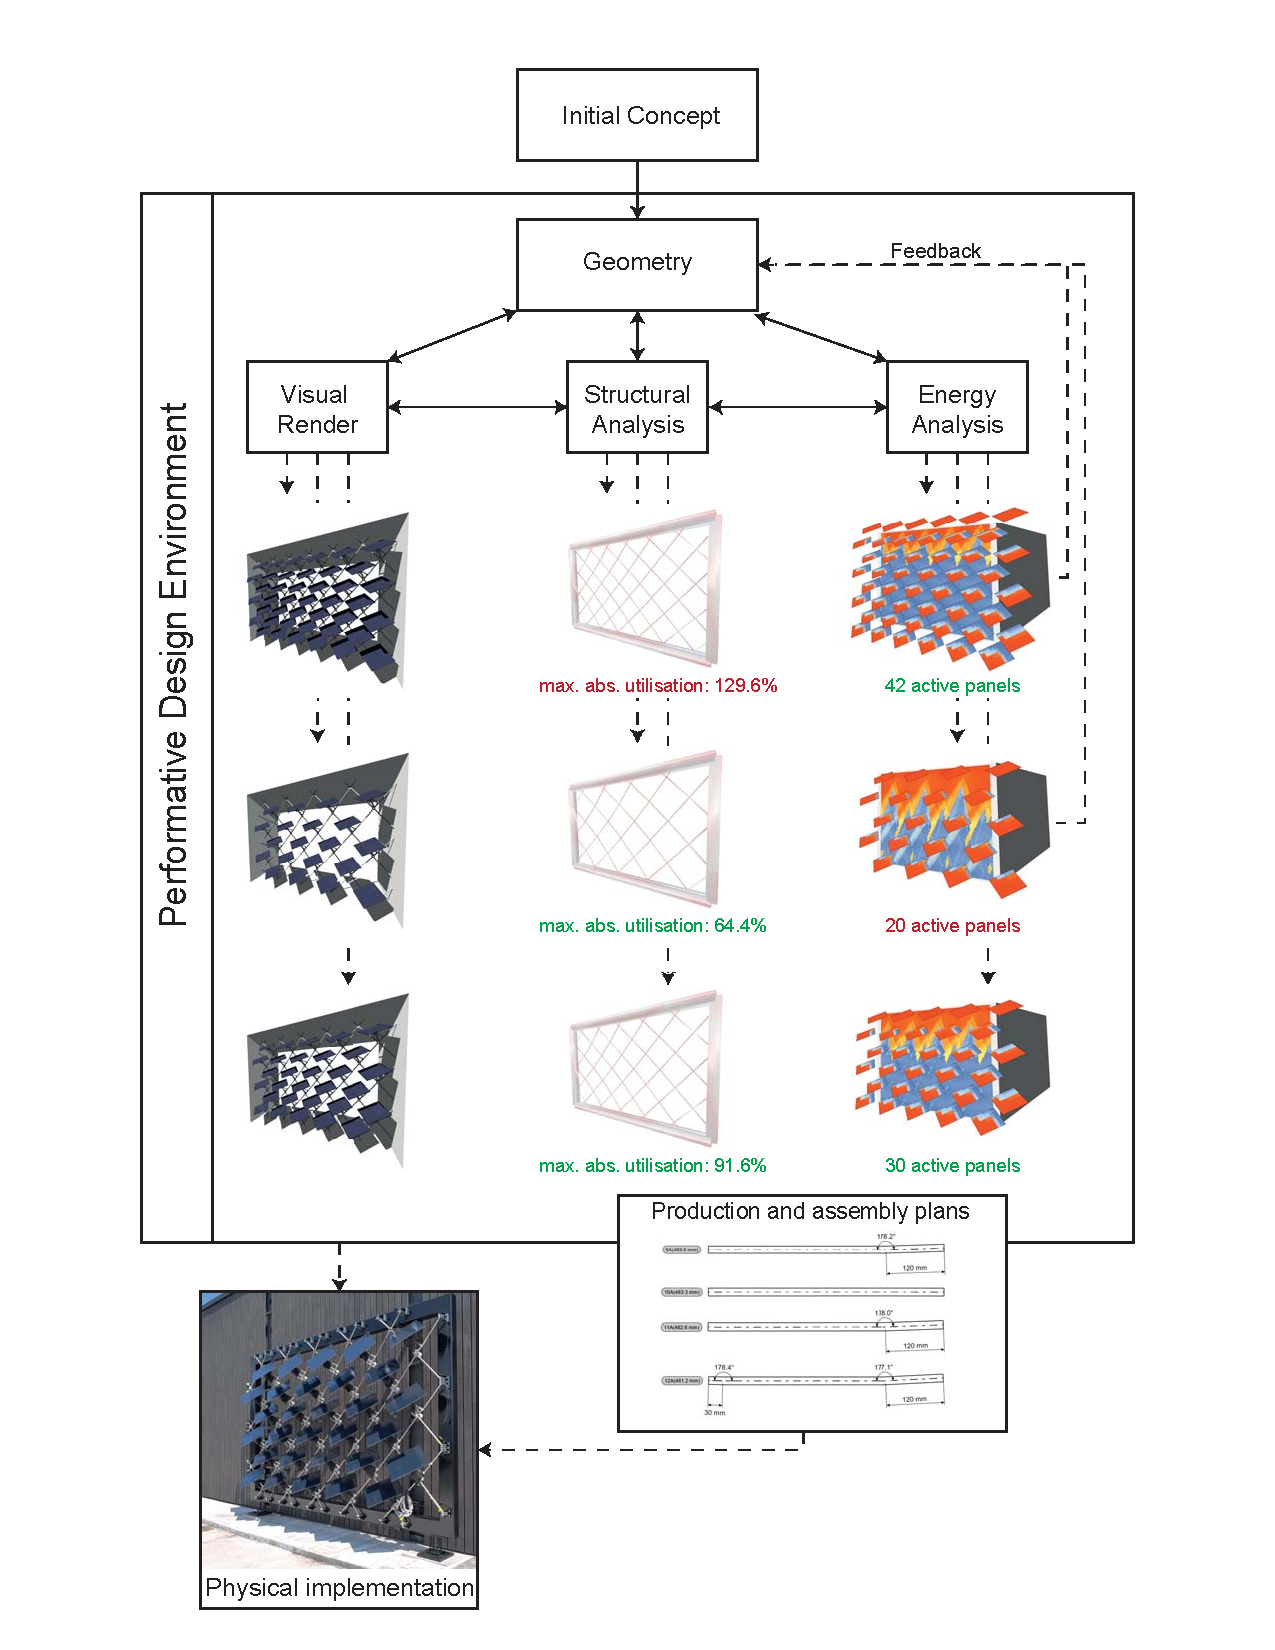
\includegraphics[width=\columnwidth, trim= 0cm 0cm 0cm 0cm,clip]{ASF_PDE_InfoGraphic.pdf}
\caption{The performative design environment is able to link four analysis methodologies for rapid design itterations}
\label{fig:performative}
\end{center}
\end{figure}

\subsection{Energy Evaluation}
\label{ch:energy}

The purpose of the ASF is to maximise electricity production on the photovoltaic (PV) panels and minimise the energy consumption of the building behind the facade. In order to best achieve this, the layout of the PV panels, and the electrical interconneciton of PV panels must be carefully designed.

The evaluation of the energetic performance of the ASF can be found in Chapter \ref{ch:asfSimulation}, and will be briefly reviewed here for completion. This part of the PDE consists of five stages: 

\begin{enumerate}
\item \textbf{Solar Radiation Model:} The radiation on the PV panels and window behind the ASF is calculated using the Grasshopper - LadyBug plugin.  \cite{roudsari2013ladybug}. An example of the simulation result is shown in Figure \ref{fig:radiation}. A tighter layout of panels allows for more PV material per facade area, however it also results in more module selfshading, which reduces the overall electricity production.
\item \textbf{PV Electricity Production:} The radiation result on the PV panels is coupled to an electrical circuit simulation of monolithically interconnected, thin-film CIGS PV modules. This model takes into account the effects of module self-shading and temperature dependence \cite{hofer2016parametric}. 
\item \textbf{Building Energy Model:} The radiation calculated on the window surface is fed to a 5R1C single zone resistance-capacitance building model based on the ISO 13790 standard \cite{de2008iso}. This calculates the heating or cooling demand of the building. A tight layout of PV panels enables more control over the solar insolation. Tight configurations tend to perform better in hot climates, whereas sparse configurations perform better in colder climates. 
\item \textbf{Daylighting Model:} A linear daylighting model based on the total flux methodology is used to determine the luminosity in the room \cite{szokolay1980handbook}. When the luminosity falls below a threshold value of 300lx, artificial lighting is turned on. Sparse configurations result in more daylight distribution, which reduces the need for artificial lighting in the morning and evening hours.
\item \textbf{Optimisation:} The simulation is conducted for all possible panel angle combinations for every hour of the year. By summing all the time steps, the annual energetic performance of the ASF can be evaluated. 
\end{enumerate}
This analysis finds the optimum balance between PV generation and daylight control to minimise heating, cooling and lighting demands where the overall objective is the minimisation of net energy.
The source code for this methodology, with installation instructions can be downloaded from github \cite{ASFGitHub,RCGitHub}.

During the design stage, this analysis is conducted for a typical day in summer, and in winter. Once a design has been selected, an annual study with hourly time steps is conducted to achieve a high resolution result.


\begin{figure}
\begin{center}
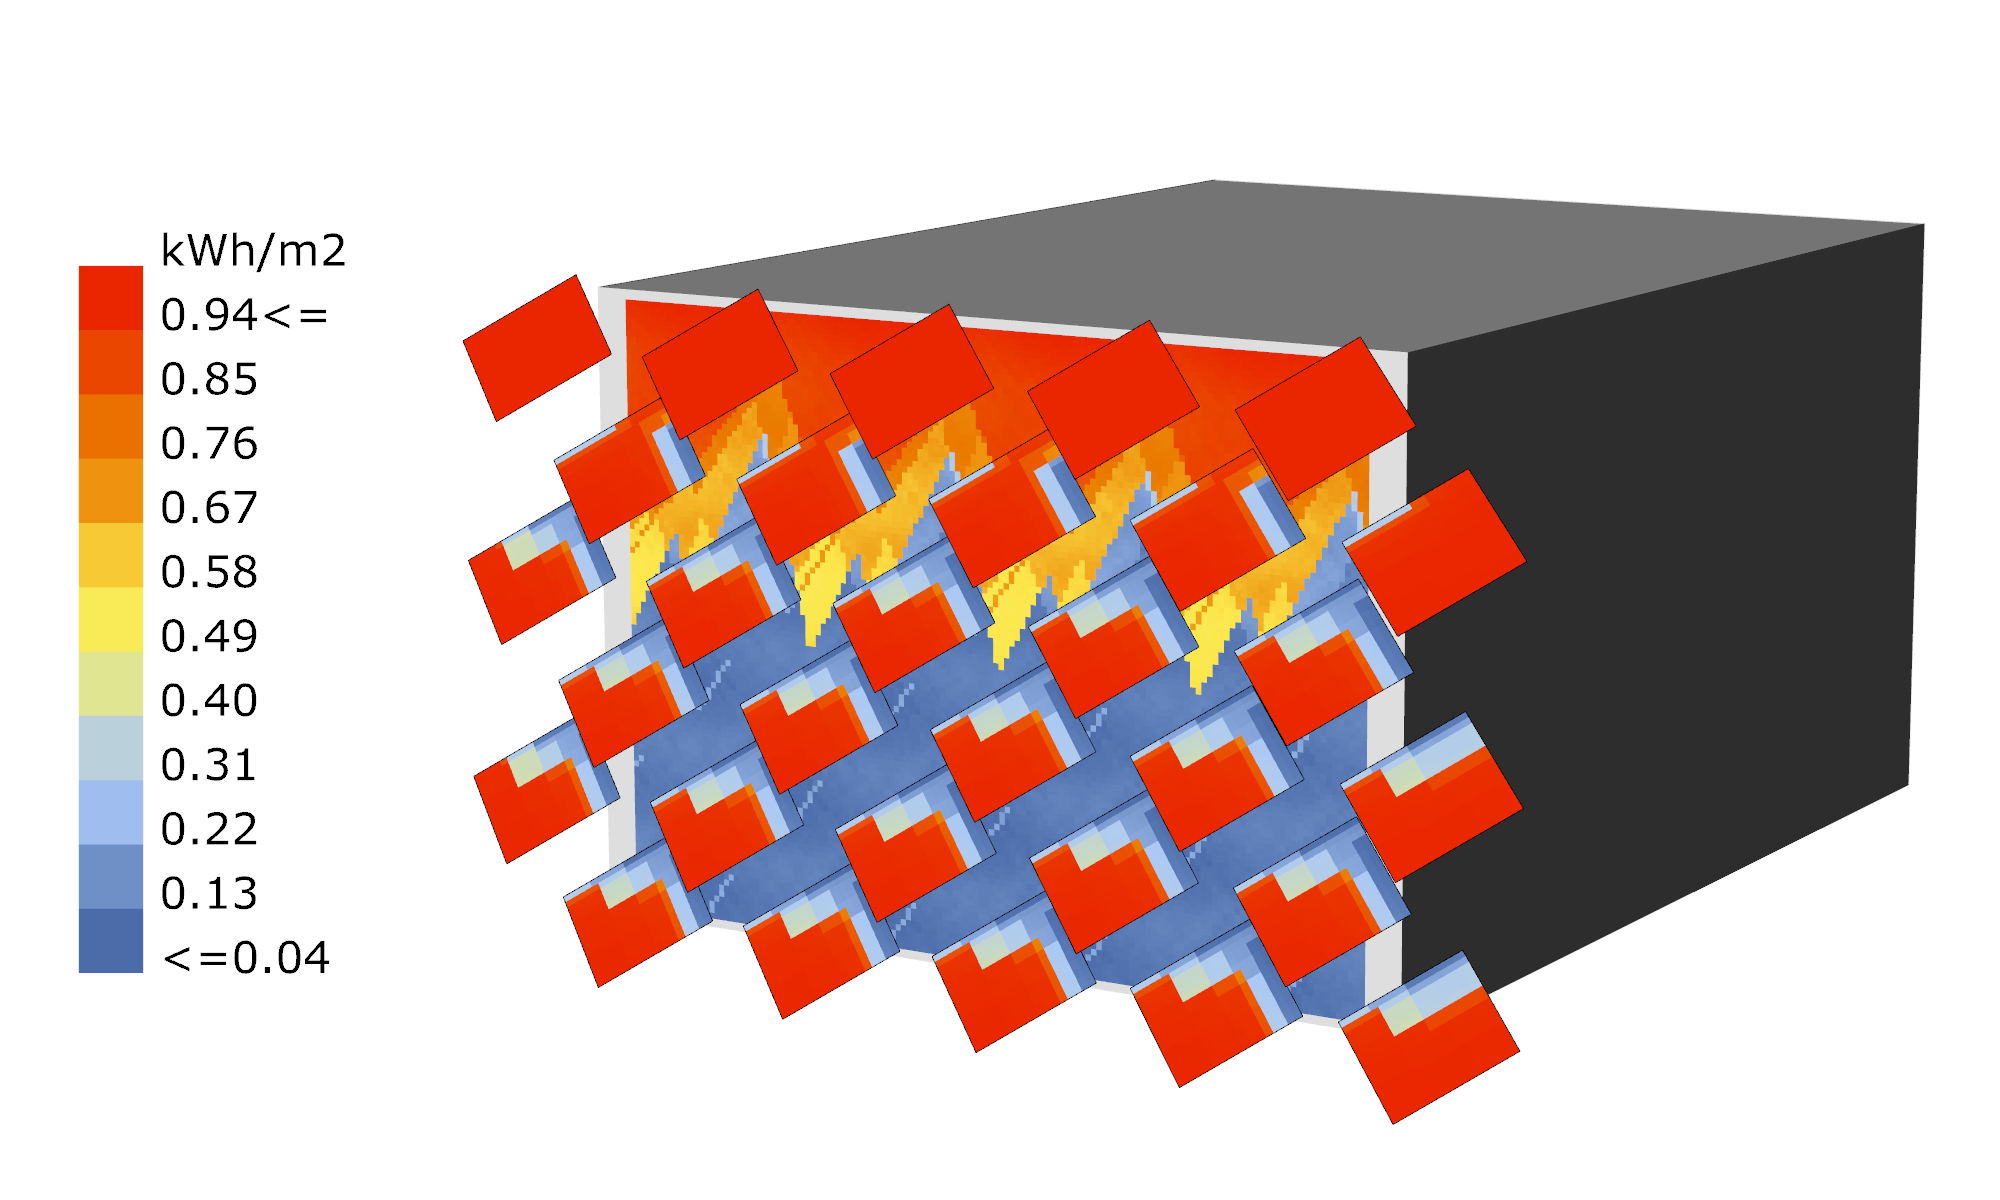
\includegraphics[width=\columnwidth, trim= 0cm 0cm 0cm 0cm,clip]{radiationHiLo2.png}
\caption{A simulation result showing the radiation on the solar panels and the window element on the 16 June 2013 between 12:00-13:00 in Zurich.}
\label{fig:radiation}
\end{center}
\end{figure}


\subsection{Structural form finding and finite element analysis}

The panel spacing, as discussed in Section \ref{ch:energy} can also influence the structural performance of the system, which in turn, influences the architectural image. It is therefore important to run the structural analysis in parallel to find the optimum solution. This subsection will first introduce the structural concept, and then detail how this concept was developed with the PDE.\\

The proposed ASF is based on a vaulted cross-hatched network of stainless steel pipes as seen in Figure \ref{fig:structure}. The junctions where the pipes cross serve as the mounting points for each dynamic photovoltaic module. All utility lines are routed within the pipe network. A steel frame supports the pipe network to create a stand-alone pre fabricated component, which can be mounted directly to the building envelope. The vaulted shape further strengthens the structure against wind loads, thus allowing for thinner pipe diameters, which increases transparency. \\


The form of the vaulted structure is determined through RhinoVault, a form finding plug in for Grasshopper \cite{Rippmann2012}. The method calculates the optimum shape of the pipe network based on the loading points and inputs to the design environment. Once the form is determined, a structural second order finite element analysis is conducted using the Karamba3d plug-in \cite{karamba} to dimension the structural elements. Further manual adjustments to the mesh can be conducted to improve the architectural image. Each manual adjustment is directly computed by the second order FEA module, providing real time feedback about the stability of the adjusted structure.  Figure \ref{fig:structureSettings} shows an example of this output with a list of simulation parameters. A load of 420N was applied on each panel node, which is equivalent to a category one hurricane on the Saffir-Simpson scale. The results are visualised in the form of coloured meshes which detail the utilisation factor in relation to the von Mises stress. A scaled down 2.2m x 1.5m prototype was constructed to validate the structural model. 

\begin{figure}
\begin{center}
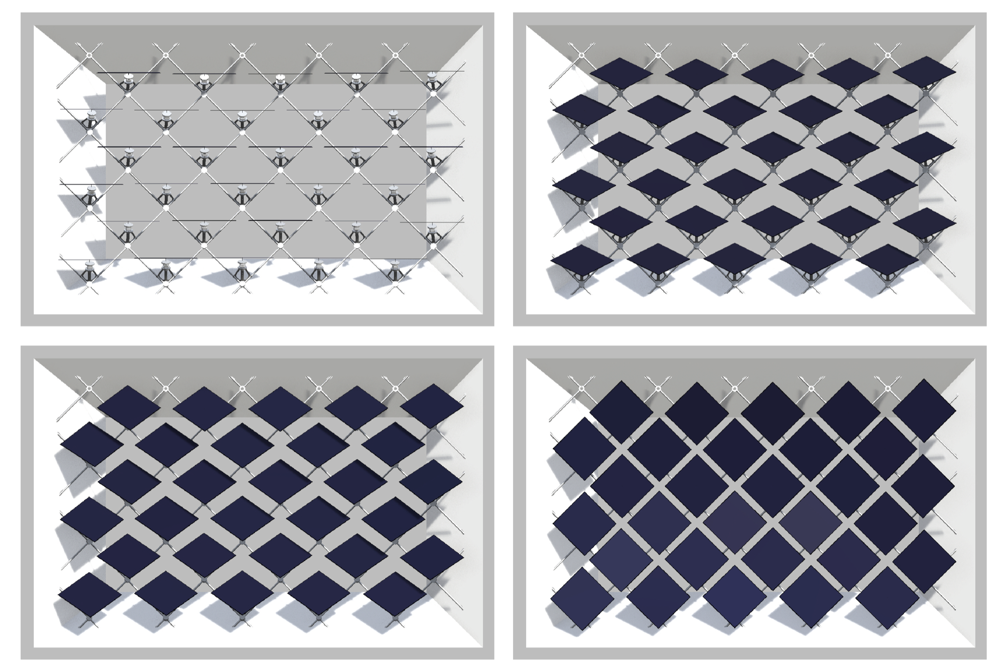
\includegraphics[width=\columnwidth, trim= 0cm 0cm 0cm 0cm,clip]{HiLoFrontRenderSmall.png}
\caption{The Adaptive Solar Facade existing in varying states}
\label{fig:structure}
\end{center}
\end{figure}

\begin{figure}
\begin{center}
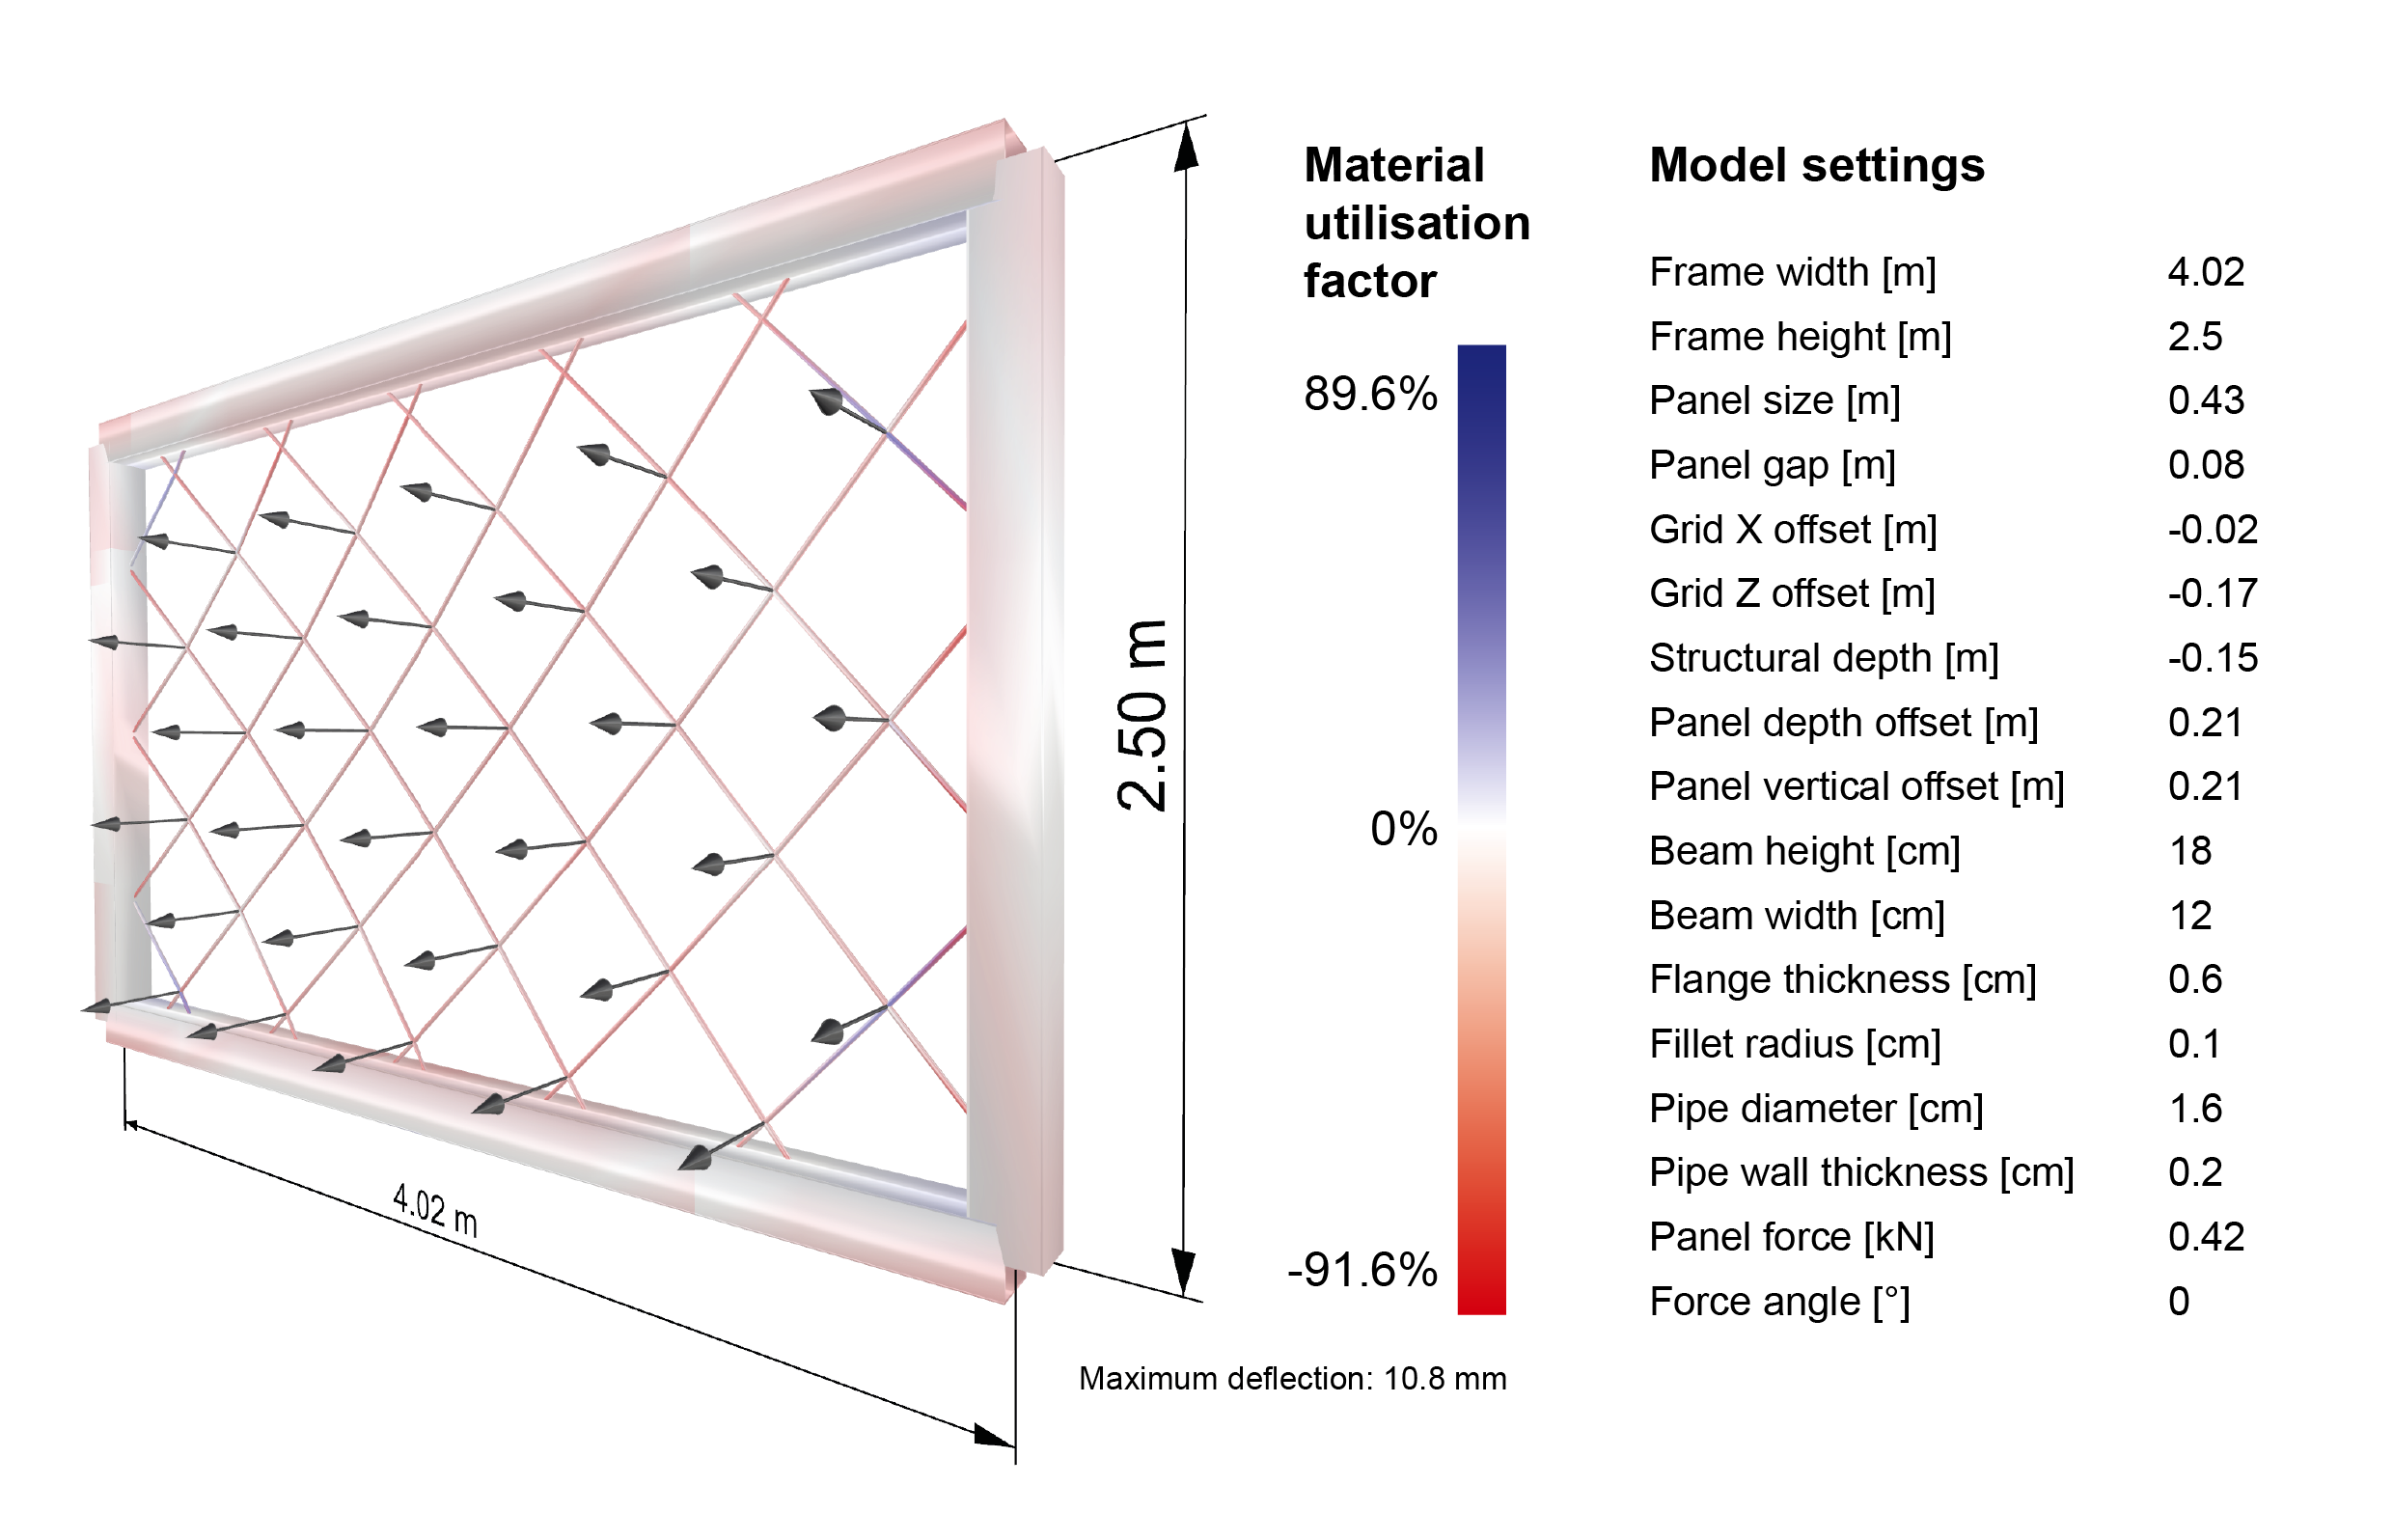
\includegraphics[width=\columnwidth, trim= 0cm 0cm 0cm 0cm,clip]{HiLo_ASF_Structural_Simulation.png}
\caption{An example output from the Karamba structural simulation. The black arrows detail the loading direction, and the colour details the utilisation factor in relation to the von Mises stress. The table on the right details the input parameters to the simulation.}
\label{fig:structureSettings}
\end{center}
\end{figure}




\subsection{Integration of classical design methods}

A purely parametric approach is very useful in investigating design possibilities, but once the concept needs to be put in practice, the parametric design environment needs to be complemented with physical prototypes, testing and classical design methods like simple 3D modelling and electronics design.
As there is a trade-off  between the  flexibility of a parameterised environment and the time required for its development, it is important to wisely choose what to parameterise and what to design with classical methods. Parametrising the entire design process of complex systems such as an ASF can result in instabilities and lead to an increase in design time. For this reason, it is important to include certain constants amongst the parametric variables. Constants include the design of the electronics, connection details, and the actuator design \cite{Svetozarevic2017a,svetozarevic2016soro}.


